%!TEX root = ../../architekturdokumentation.tex
\chapter{Backend Architektur}
	Nachfolgend werden wichtige architektonische Klassen und deren Zusammenhang im Backend mittels Klassendiagrammen beschrieben.

	\section{Klassendiagramm}
	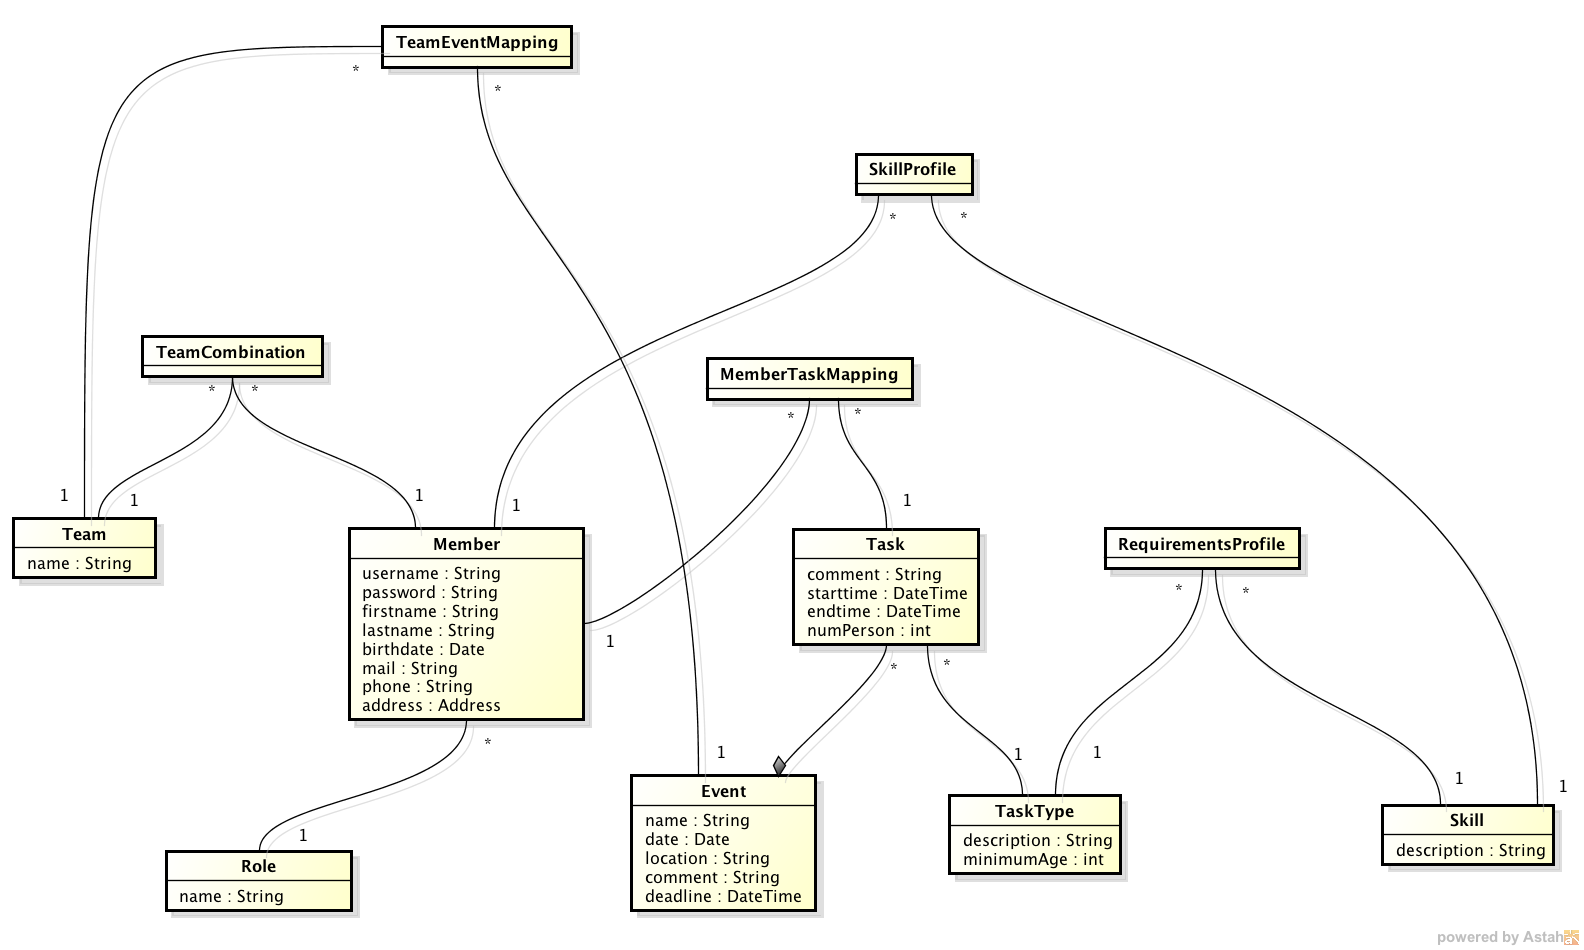
\includegraphics[width=\textwidth]{content/architekturdokumentation/images/datenmodell.png}
	
	\section{Typische Systemoperationen}

	\section{Wichtige Design Aspekte}
		\subsection{Model-View-Controller}
		Für die Presentationschicht setzen wir MVC ein, da ASP.NET eine gute Unterstützung für dieses Modell bietet. Auf alle Seiten wird mittels Controller zugegriffen. Die Views werden mithilfe der Razorsprache erstellt.

		\subsection{3-Tier-Architektur}
		Um eine möglichst hohe Abstraktion unseres Codes zu erhalten, haben wir uns für eine 3-Tier-Architektur entschieden, die unsere Applikation in die drei Schichten Web, Service und DataAccesLayer (Dal) unterteilt. Alle Datenbankspezifischen Operationen sollen im DAL Layer vorgenommen werden. Alle Zugriffe aus dem Web sollen über die Web-Schicht behandelt werden. Die Zugriffe auf externe Schnittstellen über den Service-Layer

		\subsection{Entity Framework Code-First}
		Gemäss den Empfehlungen von Microsoft, soll für neue Projekte Code First eingesetzt werden. In diesem Konzept wird das Datenbankmodell direkt durch den C# Code generiert. Dies bietet uns den Vorteil dass man nur noch mit C# arbeiten muss.